\section{Descrição funcional} % (fold)
\label{sec:descricaofuncional}
\begin{figure}[!htb]
  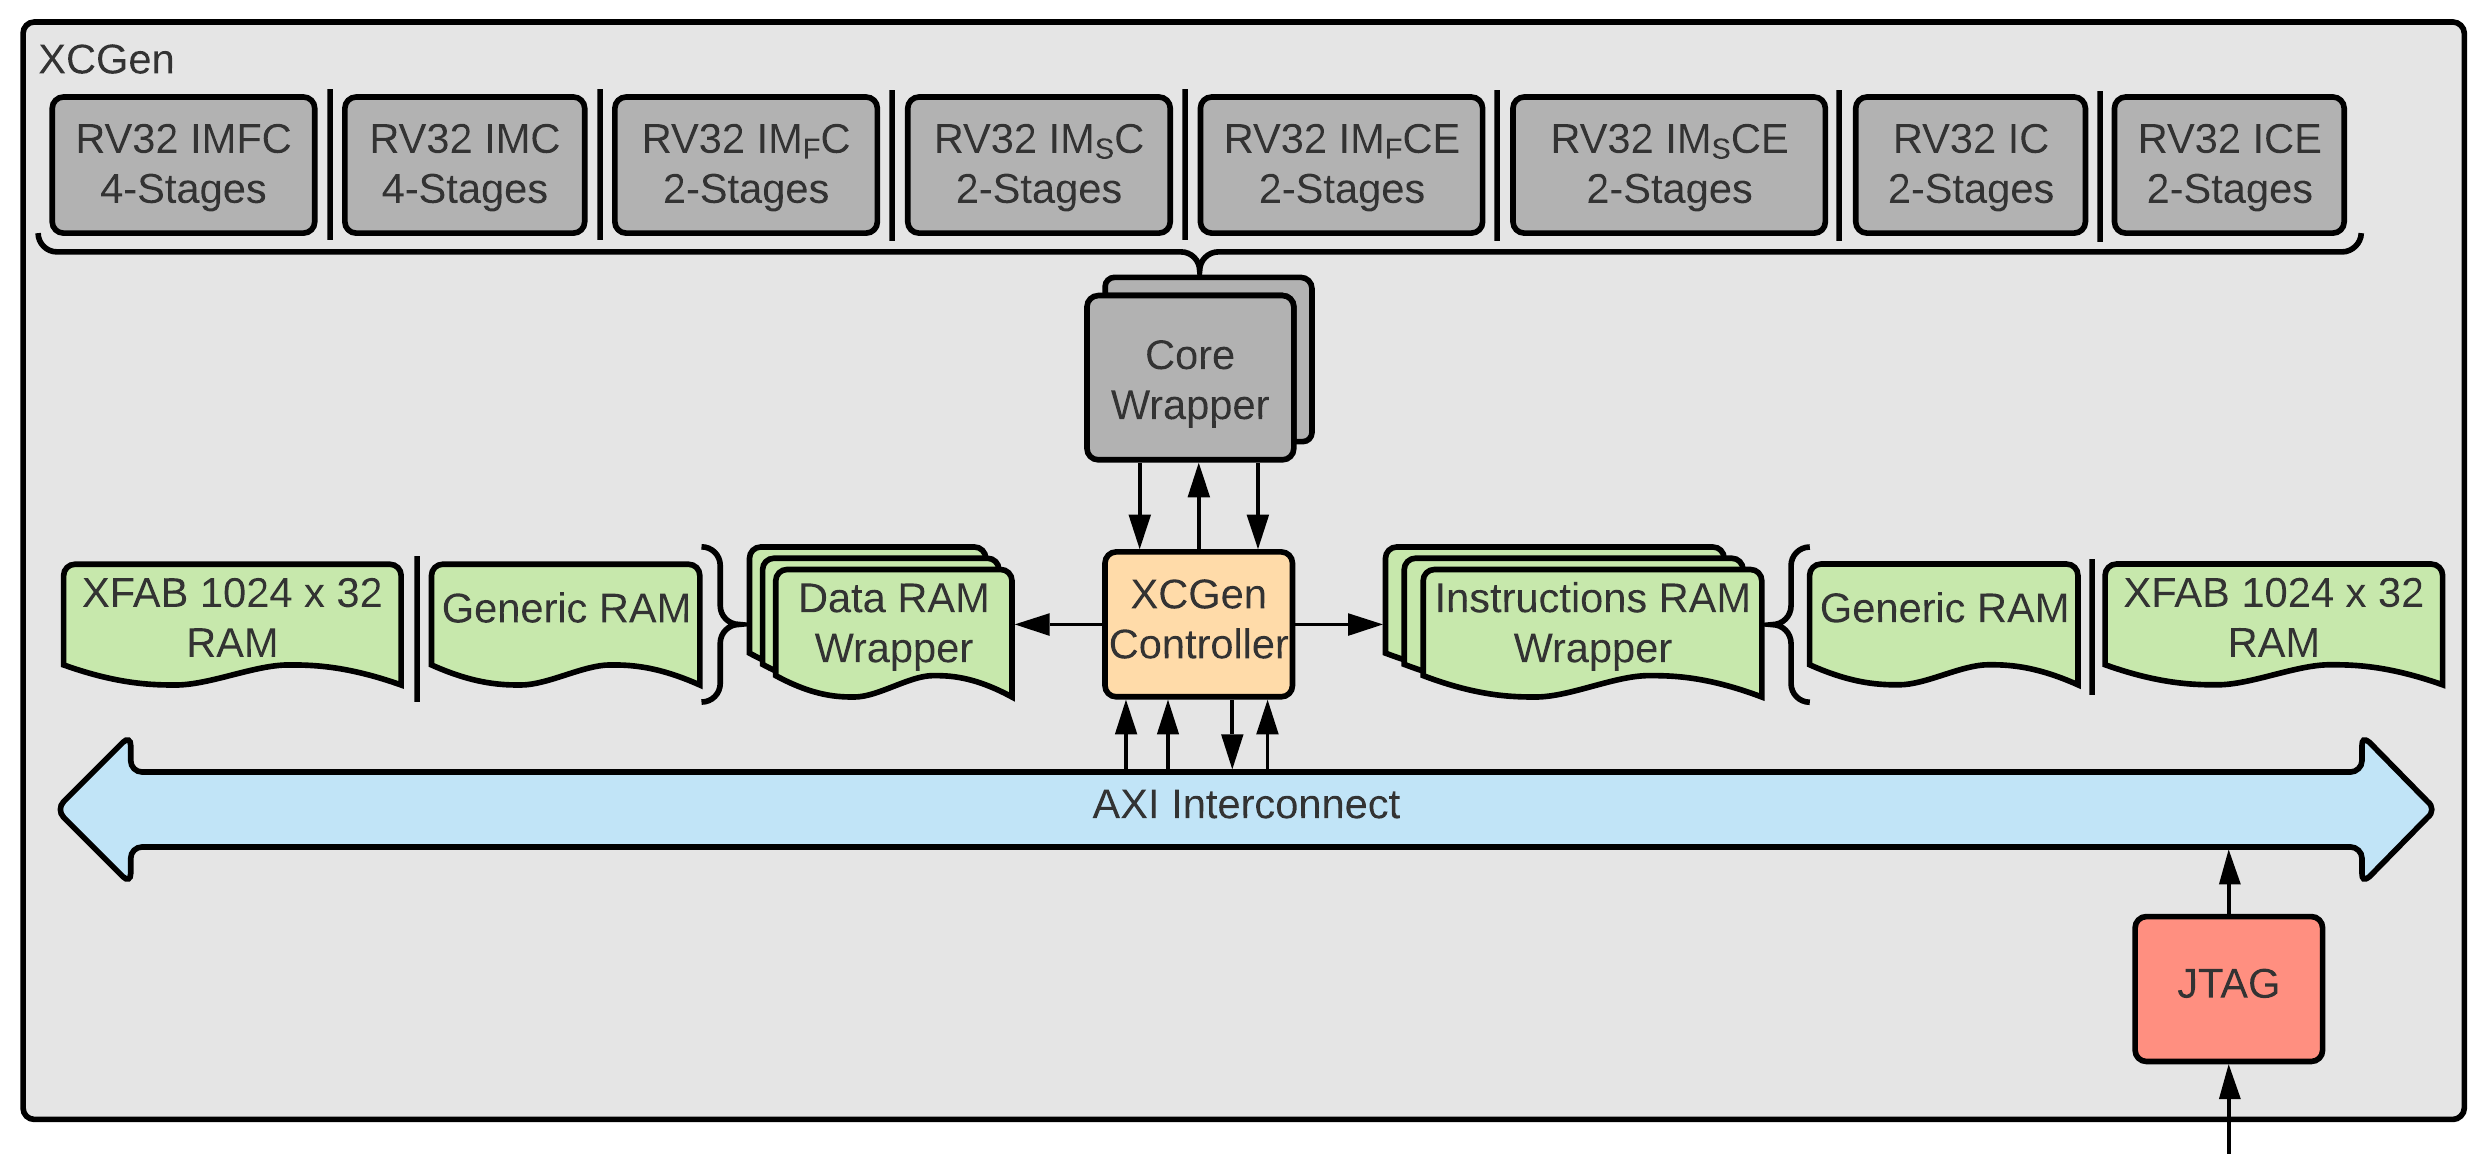
\includegraphics[width=\linewidth]{diagrams/XCGen2.png}
  \caption{Diagrama do XCGen.}
  \label{fig:top}
\end{figure}

\subsection{XCGen}
Através do uso dos parametros, é possível adicionar blocos ao SoC, como pode ser visto na imagem abaixo;
\begin{figure}[!htb]
  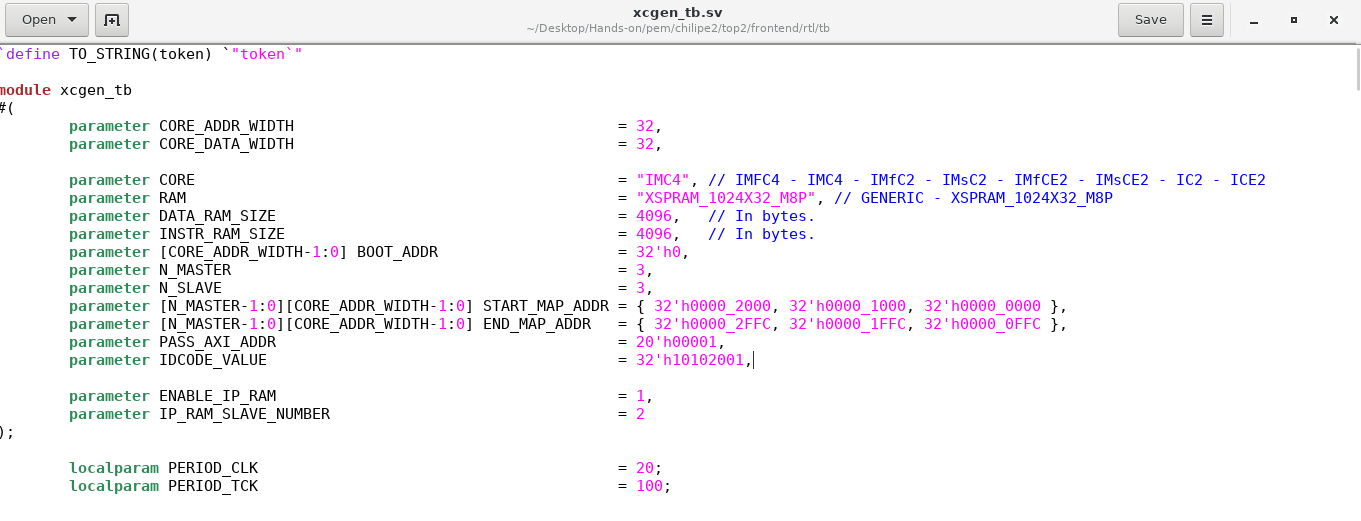
\includegraphics[width=\linewidth]{diagrams/tb.png}
  \caption{parametros do topo/tb.}
  \label{fig:top}
\end{figure}
\\
\begin{itemize}
  \item Alterando o número de mestres e escravos, é possível alterar a quantidade dos mesmos, no sistema;
  \item Possível alterar o tipo de processador(CORE);
  \item Possível alterar o tipo de memória(RAM)entre a  xfab e genérica(não sistetisável);
  \item atualmente é possível adicionar um IP generico, e definir o escravo(SLAVE) responsável pelo menos(ENABLE\_ IP\_RAM);
  \item É possível declarar qual dos escravos será responsável pelo novo IP(IP\_ RAM \_ SLAVE \_NUMBER);
  \item Total controle do mapa de memória do AXI(START/END\_ MAP \_ ADDR) ;
\end{itemize}

Na figura abaixo pode ser visto, como são adicionados novos blocos, através de generate, neste caso é o "generic\_ip":
\begin{figure}[!htb]
  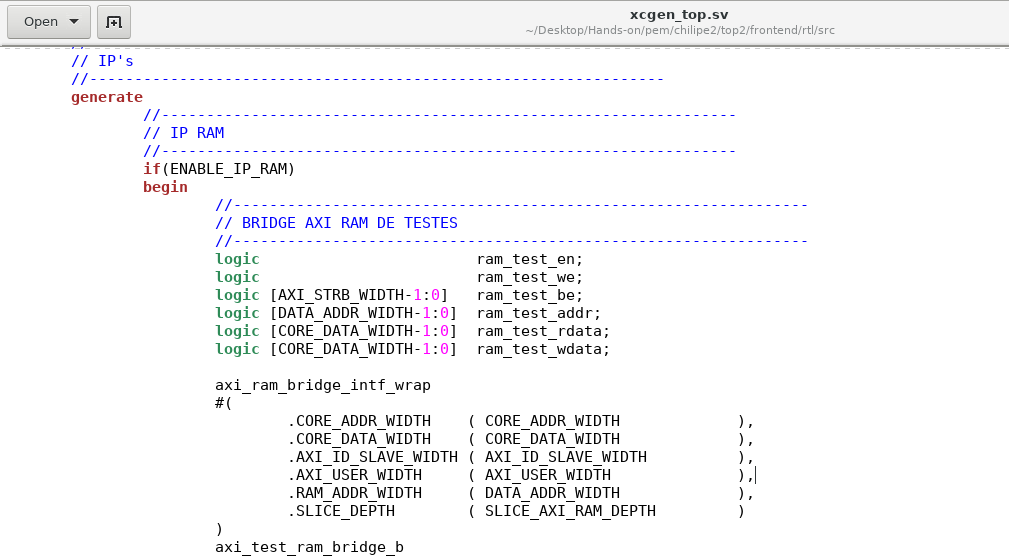
\includegraphics[width=\linewidth]{diagrams/ex_generate.png}
  \caption{Exemplo do uso de Generate.}
  \label{fig:top}
\end{figure}
\\
\subsection{CORE}
Core consiste no conjunto de processadores suportados pelo sistema, em comum eles possuem uma conexao direta as memórias de instrução e dados, e fazem o fetch, na memória de instruções, após o sinal fetch\_ enable\_i obter o valor "1";
A função do processador é executar instruções, utilizando o padrão da ISA risc\-v;

\subsection{JTAG}
O JTAG é responsável por fazer escrita e leitura nos registradores do SoC, ele faz isso através de uma entrada  e sáida serial, a qual o usuário tem acesso;
\begin{figure}[H]
  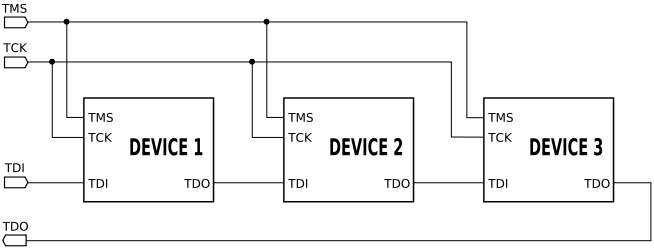
\includegraphics[width=\linewidth]{diagrams/jtag.png}
  \caption{jtag interface.}
  \label{fig:top}
\end{figure}

\subsection{AXI}
O AXI é responsável por conectar todos os mestres e escravos do sistema, através de uma interface em comum, e cada IP que não esteja neste padrão de sinais, possue uma bridge de tradução, para consolidar essa comunicação;
O AXI realiza transações através de um conjunto de handshakes  (valid,ready) para garantir que a informação chegou ao seu destino;
Possue 5 interfaces:

\begin{itemize}
  \item AW(address write): Consiste no endereço e seus sinais, onde se quer escrever uma informação;
  \item W(write):Consiste na informação a qual se quer escrever no endereço;
  \item B(response):Sinais de resposta a leitura;
  \item AR(address read):Consiste no endereço e seus sinais, onde se quer ler os dados;
  \item R(read):Consiste do dado a ser lido e seus sinais;
\end{itemize}
O AXI possue total controle para alterar o mapa de memória com os sinais:
\begin{itemize}
  \item start\_ add\_i : Endereço inicial de cada escravo(slave) do sistema;
  \item end\_ add\_i : Endereço final de cada escravo(slave) do sistema;
\end{itemize}
\begin{figure}[H]
  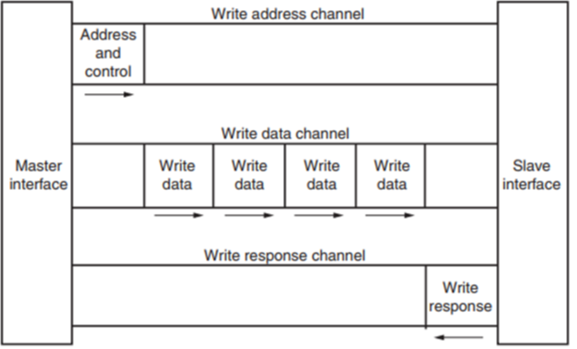
\includegraphics[width=\linewidth]{diagrams/axi comunication.png}
  \caption{Exemplo de transação axi.}
  \label{fig:top}
\end{figure}
\subsection{Tool chain}
É o a interface de software utilizada para geração de instruções em assembly(a ser interpretadas pelo core) através de uma linguágem de alto nível(c);
\begin{figure}[H]
  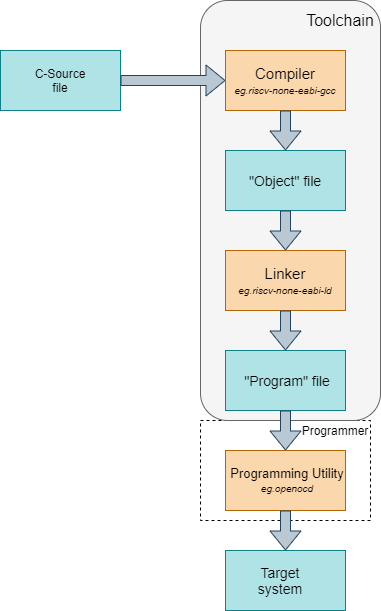
\includegraphics[width=\linewidth]{diagrams/toolchain.png}
  \caption{Fluxo da toolchain.}
  \label{fig:top}
\end{figure}
% section descricaofuncional (end)
